\documentclass[1p]{elsarticle_modified}
%\bibliographystyle{elsarticle-num}

%\usepackage[colorlinks]{hyperref}
%\usepackage{abbrmath_seonhwa} %\Abb, \Ascr, \Acal ,\Abf, \Afrak
\usepackage{amsfonts}
\usepackage{amssymb}
\usepackage{amsmath}
\usepackage{amsthm}
\usepackage{scalefnt}
\usepackage{amsbsy}
\usepackage{kotex}
\usepackage{caption}
\usepackage{subfig}
\usepackage{color}
\usepackage{graphicx}
\usepackage{xcolor} %% white, black, red, green, blue, cyan, magenta, yellow
\usepackage{float}
\usepackage{setspace}
\usepackage{hyperref}

\usepackage{tikz}
\usetikzlibrary{arrows}

\usepackage{multirow}
\usepackage{array} % fixed length table
\usepackage{hhline}

%%%%%%%%%%%%%%%%%%%%%
\makeatletter
\renewcommand*\env@matrix[1][\arraystretch]{%
	\edef\arraystretch{#1}%
	\hskip -\arraycolsep
	\let\@ifnextchar\new@ifnextchar
	\array{*\c@MaxMatrixCols c}}
\makeatother %https://tex.stackexchange.com/questions/14071/how-can-i-increase-the-line-spacing-in-a-matrix
%%%%%%%%%%%%%%%

\usepackage[normalem]{ulem}

\newcommand{\msout}[1]{\ifmmode\text{\sout{\ensuremath{#1}}}\else\sout{#1}\fi}
%SOURCE: \msout is \stkout macro in https://tex.stackexchange.com/questions/20609/strikeout-in-math-mode

\newcommand{\cancel}[1]{
	\ifmmode
	{\color{red}\msout{#1}}
	\else
	{\color{red}\sout{#1}}
	\fi
}

\newcommand{\add}[1]{
	{\color{blue}\uwave{#1}}
}

\newcommand{\replace}[2]{
	\ifmmode
	{\color{red}\msout{#1}}{\color{blue}\uwave{#2}}
	\else
	{\color{red}\sout{#1}}{\color{blue}\uwave{#2}}
	\fi
}

\newcommand{\Sol}{\mathcal{S}} %segment
\newcommand{\D}{D} %diagram
\newcommand{\A}{\mathcal{A}} %arc


%%%%%%%%%%%%%%%%%%%%%%%%%%%%%5 test

\def\sl{\operatorname{\textup{SL}}(2,\Cbb)}
\def\psl{\operatorname{\textup{PSL}}(2,\Cbb)}
\def\quan{\mkern 1mu \triangleright \mkern 1mu}

\theoremstyle{definition}
\newtheorem{thm}{Theorem}[section]
\newtheorem{prop}[thm]{Proposition}
\newtheorem{lem}[thm]{Lemma}
\newtheorem{ques}[thm]{Question}
\newtheorem{cor}[thm]{Corollary}
\newtheorem{defn}[thm]{Definition}
\newtheorem{exam}[thm]{Example}
\newtheorem{rmk}[thm]{Remark}
\newtheorem{alg}[thm]{Algorithm}

\newcommand{\I}{\sqrt{-1}}
\begin{document}

%\begin{frontmatter}
%
%\title{Boundary parabolic representations of knots up to 8 crossings}
%
%%% Group authors per affiliation:
%\author{Yunhi Cho} 
%\address{Department of Mathematics, University of Seoul, Seoul, Korea}
%\ead{yhcho@uos.ac.kr}
%
%
%\author{Seonhwa Kim} %\fnref{s_kim}}
%\address{Center for Geometry and Physics, Institute for Basic Science, Pohang, 37673, Korea}
%\ead{ryeona17@ibs.re.kr}
%
%\author{Hyuk Kim}
%\address{Department of Mathematical Sciences, Seoul National University, Seoul 08826, Korea}
%\ead{hyukkim@snu.ac.kr}
%
%\author{Seokbeom Yoon}
%\address{Department of Mathematical Sciences, Seoul National University, Seoul, 08826,  Korea}
%\ead{sbyoon15@snu.ac.kr}
%
%\begin{abstract}
%We find all boundary parabolic representation of knots up to 8 crossings.
%
%\end{abstract}
%\begin{keyword}
%    \MSC[2010] 57M25 
%\end{keyword}
%
%\end{frontmatter}

%\linenumbers
%\tableofcontents
%
\newcommand\colored[1]{\textcolor{white}{\rule[-0.35ex]{0.8em}{1.4ex}}\kern-0.8em\color{red} #1}%
%\newcommand\colored[1]{\textcolor{white}{ #1}\kern-2.17ex	\textcolor{white}{ #1}\kern-1.81ex	\textcolor{white}{ #1}\kern-2.15ex\color{red}#1	}

{\Large $\underline{12n_{0714}~(K12n_{0714})}$}

\setlength{\tabcolsep}{10pt}
\renewcommand{\arraystretch}{1.6}
\vspace{1cm}\begin{tabular}{m{100pt}>{\centering\arraybackslash}m{274pt}}
\multirow{5}{120pt}{
	\centering
	\includegraphics[width=112pt]{../../../GIT/diagram.site/Diagrams/png/2803_12n_0714.png}\\
\ \ \ A knot diagram\footnotemark}&
\allowdisplaybreaks
\textbf{Linearized knot diagam} \\
\cline{2-2}
 &
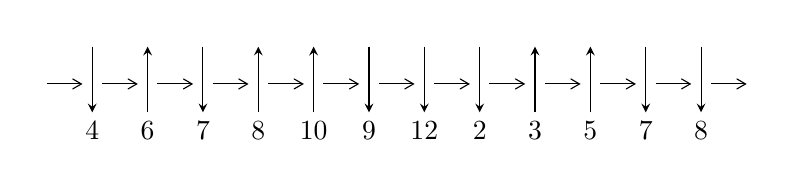
\begin{tikzpicture}[x=20pt, y=17pt]
	% nodes
	\node (C0) at (0, 0) {};
	\node (C1) at (1, 0) {};
	\node (C1U) at (1, +1) {};
	\node (C1D) at (1, -1) {4};

	\node (C2) at (2, 0) {};
	\node (C2U) at (2, +1) {};
	\node (C2D) at (2, -1) {6};

	\node (C3) at (3, 0) {};
	\node (C3U) at (3, +1) {};
	\node (C3D) at (3, -1) {7};

	\node (C4) at (4, 0) {};
	\node (C4U) at (4, +1) {};
	\node (C4D) at (4, -1) {8};

	\node (C5) at (5, 0) {};
	\node (C5U) at (5, +1) {};
	\node (C5D) at (5, -1) {10};

	\node (C6) at (6, 0) {};
	\node (C6U) at (6, +1) {};
	\node (C6D) at (6, -1) {9};

	\node (C7) at (7, 0) {};
	\node (C7U) at (7, +1) {};
	\node (C7D) at (7, -1) {12};

	\node (C8) at (8, 0) {};
	\node (C8U) at (8, +1) {};
	\node (C8D) at (8, -1) {2};

	\node (C9) at (9, 0) {};
	\node (C9U) at (9, +1) {};
	\node (C9D) at (9, -1) {3};

	\node (C10) at (10, 0) {};
	\node (C10U) at (10, +1) {};
	\node (C10D) at (10, -1) {5};

	\node (C11) at (11, 0) {};
	\node (C11U) at (11, +1) {};
	\node (C11D) at (11, -1) {7};

	\node (C12) at (12, 0) {};
	\node (C12U) at (12, +1) {};
	\node (C12D) at (12, -1) {8};
	\node (C13) at (13, 0) {};

	% arrows
	\draw[->,>={angle 60}]
	(C0) edge (C1) (C1) edge (C2) (C2) edge (C3) (C3) edge (C4) (C4) edge (C5) (C5) edge (C6) (C6) edge (C7) (C7) edge (C8) (C8) edge (C9) (C9) edge (C10) (C10) edge (C11) (C11) edge (C12) (C12) edge (C13) ;	\draw[->,>=stealth]
	(C1U) edge (C1D) (C2D) edge (C2U) (C3U) edge (C3D) (C4D) edge (C4U) (C5D) edge (C5U) (C6U) edge (C6D) (C7U) edge (C7D) (C8U) edge (C8D) (C9D) edge (C9U) (C10D) edge (C10U) (C11U) edge (C11D) (C12U) edge (C12D) ;
	\end{tikzpicture} \\
\hhline{~~} \\& 
\textbf{Solving Sequence} \\ \cline{2-2} 
 &
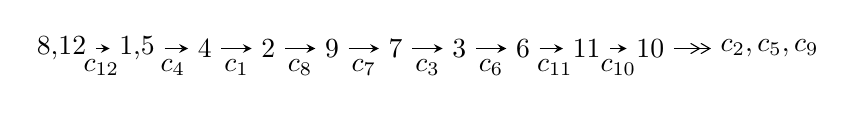
\begin{tikzpicture}[x=23pt, y=7pt]
	% node
	\node (A0) at (-1/8, 0) {8,12};
	\node (A1) at (17/16, 0) {1,5};
	\node (A2) at (17/8, 0) {4};
	\node (A3) at (25/8, 0) {2};
	\node (A4) at (33/8, 0) {9};
	\node (A5) at (41/8, 0) {7};
	\node (A6) at (49/8, 0) {3};
	\node (A7) at (57/8, 0) {6};
	\node (A8) at (65/8, 0) {11};
	\node (A9) at (73/8, 0) {10};
	\node (C1) at (1/2, -1) {$c_{12}$};
	\node (C2) at (13/8, -1) {$c_{4}$};
	\node (C3) at (21/8, -1) {$c_{1}$};
	\node (C4) at (29/8, -1) {$c_{8}$};
	\node (C5) at (37/8, -1) {$c_{7}$};
	\node (C6) at (45/8, -1) {$c_{3}$};
	\node (C7) at (53/8, -1) {$c_{6}$};
	\node (C8) at (61/8, -1) {$c_{11}$};
	\node (C9) at (69/8, -1) {$c_{10}$};
	\node (A10) at (11, 0) {$c_{2},c_{5},c_{9}$};

	% edge
	\draw[->,>=stealth]	
	(A0) edge (A1) (A1) edge (A2) (A2) edge (A3) (A3) edge (A4) (A4) edge (A5) (A5) edge (A6) (A6) edge (A7) (A7) edge (A8) (A8) edge (A9) ;
	\draw[->>,>={angle 60}]	
	(A9) edge (A10);
\end{tikzpicture} \\ 

\end{tabular} \\

\footnotetext{
The image of knot diagram is generated by the software ``\textbf{Draw programme}" developed by Andrew Bartholomew(\url{http://www.layer8.co.uk/maths/draw/index.htm\#Running-draw}), where we modified some parts for our purpose(\url{https://github.com/CATsTAILs/LinksPainter}).
}\phantom \\ \newline 
\centering \textbf{Ideals for irreducible components\footnotemark of $X_{\text{par}}$} 
 
\begin{align*}
I^u_{1}&=\langle 
-4.87692\times10^{258} u^{86}+7.24779\times10^{258} u^{85}+\cdots+2.73086\times10^{260} b+1.29464\times10^{261},\\
\phantom{I^u_{1}}&\phantom{= \langle  }-3.32833\times10^{258} u^{86}+1.03709\times10^{259} u^{85}+\cdots+2.73086\times10^{260} a+2.37253\times10^{261},\\
\phantom{I^u_{1}}&\phantom{= \langle  }u^{87}- u^{86}+\cdots-144 u+67\rangle \\
I^u_{2}&=\langle 
-32933031018 u^{21}+1113442853 u^{20}+\cdots+9952263913 b-142566726414,\\
\phantom{I^u_{2}}&\phantom{= \langle  }-32258549399 u^{21}+13152988225 u^{20}+\cdots+9952263913 a+5817215377,\\
\phantom{I^u_{2}}&\phantom{= \langle  }u^{22}-8 u^{20}+\cdots+7 u+1\rangle \\
\\
\end{align*}
\raggedright * 2 irreducible components of $\dim_{\mathbb{C}}=0$, with total 109 representations.\\
\footnotetext{All coefficients of polynomials are rational numbers. But the coefficients are sometimes approximated in decimal forms when there is not enough margin.}
\newpage
\renewcommand{\arraystretch}{1}
\centering \section*{I. $I^u_{1}= \langle -4.88\times10^{258} u^{86}+7.25\times10^{258} u^{85}+\cdots+2.73\times10^{260} b+1.29\times10^{261},\;-3.33\times10^{258} u^{86}+1.04\times10^{259} u^{85}+\cdots+2.73\times10^{260} a+2.37\times10^{261},\;u^{87}- u^{86}+\cdots-144 u+67 \rangle$}
\flushleft \textbf{(i) Arc colorings}\\
\begin{tabular}{m{7pt} m{180pt} m{7pt} m{180pt} }
\flushright $a_{8}=$&$\begin{pmatrix}0\\u\end{pmatrix}$ \\
\flushright $a_{12}=$&$\begin{pmatrix}1\\0\end{pmatrix}$ \\
\flushright $a_{1}=$&$\begin{pmatrix}1\\u^2\end{pmatrix}$ \\
\flushright $a_{5}=$&$\begin{pmatrix}0.0121878 u^{86}-0.0379766 u^{85}+\cdots+3.72518 u-8.68785\\0.0178585 u^{86}-0.0265403 u^{85}+\cdots-4.57034 u-4.74075\end{pmatrix}$ \\
\flushright $a_{4}=$&$\begin{pmatrix}0.0121878 u^{86}-0.0379766 u^{85}+\cdots+3.72518 u-8.68785\\-0.0308890 u^{86}-0.0224193 u^{85}+\cdots-9.10052 u-3.01290\end{pmatrix}$ \\
\flushright $a_{2}=$&$\begin{pmatrix}0.0204608 u^{86}-0.00597308 u^{85}+\cdots-3.14988 u-2.22578\\0.0389753 u^{86}+0.00472462 u^{85}+\cdots+15.9789 u+3.97260\end{pmatrix}$ \\
\flushright $a_{9}=$&$\begin{pmatrix}0.00754574 u^{86}+0.00780789 u^{85}+\cdots-1.85076 u-0.0940809\\0.0253749 u^{86}+0.0235466 u^{85}+\cdots+15.0954 u+6.13843\end{pmatrix}$ \\
\flushright $a_{7}=$&$\begin{pmatrix}u\\u\end{pmatrix}$ \\
\flushright $a_{3}=$&$\begin{pmatrix}0.0132086 u^{86}-0.0308291 u^{85}+\cdots+2.64852 u-6.84404\\-0.0298682 u^{86}-0.0152718 u^{85}+\cdots-10.1772 u-1.16910\end{pmatrix}$ \\
\flushright $a_{6}=$&$\begin{pmatrix}-0.0197591 u^{86}+0.0413246 u^{85}+\cdots+7.85051 u+9.58494\\0.0940033 u^{86}-0.0539560 u^{85}+\cdots+28.9246 u-17.1001\end{pmatrix}$ \\
\flushright $a_{11}=$&$\begin{pmatrix}- u^2+1\\- u^2\end{pmatrix}$ \\
\flushright $a_{10}=$&$\begin{pmatrix}0.222309 u^{86}-0.106889 u^{85}+\cdots+14.9456 u-23.4599\\0.00662288 u^{86}+0.0179377 u^{85}+\cdots+12.6317 u+6.50996\end{pmatrix}$\\&\end{tabular}
\flushleft \textbf{(ii) Obstruction class $= -1$}\\~\\
\flushleft \textbf{(iii) Cusp Shapes $= 0.0570476 u^{86}+0.180502 u^{85}+\cdots+46.1820 u+3.78747$}\\~\\
\newpage\renewcommand{\arraystretch}{1}
\flushleft \textbf{(iv) u-Polynomials at the component}\newline \\
\begin{tabular}{m{50pt}|m{274pt}}
Crossings & \hspace{64pt}u-Polynomials at each crossing \\
\hline $$\begin{aligned}c_{1}\end{aligned}$$&$\begin{aligned}
&u^{87}+3 u^{86}+\cdots+3937 u+511
\end{aligned}$\\
\hline $$\begin{aligned}c_{2}\end{aligned}$$&$\begin{aligned}
&u^{87}-5 u^{86}+\cdots-2768 u-437
\end{aligned}$\\
\hline $$\begin{aligned}c_{3}\end{aligned}$$&$\begin{aligned}
&u^{87}-3 u^{86}+\cdots-4842 u-1687
\end{aligned}$\\
\hline $$\begin{aligned}c_{4}\end{aligned}$$&$\begin{aligned}
&u^{87}- u^{86}+\cdots+5250 u+811
\end{aligned}$\\
\hline $$\begin{aligned}c_{5},c_{10}\end{aligned}$$&$\begin{aligned}
&u^{87}- u^{86}+\cdots+833881 u+81631
\end{aligned}$\\
\hline $$\begin{aligned}c_{6}\end{aligned}$$&$\begin{aligned}
&u^{87}- u^{86}+\cdots+46 u-7
\end{aligned}$\\
\hline $$\begin{aligned}c_{7},c_{11},c_{12}\end{aligned}$$&$\begin{aligned}
&u^{87}- u^{86}+\cdots-144 u+67
\end{aligned}$\\
\hline $$\begin{aligned}c_{8}\end{aligned}$$&$\begin{aligned}
&u^{87}-2 u^{86}+\cdots-5106 u+38332
\end{aligned}$\\
\hline $$\begin{aligned}c_{9}\end{aligned}$$&$\begin{aligned}
&u^{87}-2 u^{86}+\cdots+58 u+7
\end{aligned}$\\
\hline
\end{tabular}\\~\\
\newpage\renewcommand{\arraystretch}{1}
\flushleft \textbf{(v) Riley Polynomials at the component}\newline \\
\begin{tabular}{m{50pt}|m{274pt}}
Crossings & \hspace{64pt}Riley Polynomials at each crossing \\
\hline $$\begin{aligned}c_{1}\end{aligned}$$&$\begin{aligned}
&y^{87}+67 y^{86}+\cdots-8202255 y-261121
\end{aligned}$\\
\hline $$\begin{aligned}c_{2}\end{aligned}$$&$\begin{aligned}
&y^{87}+31 y^{86}+\cdots-9342720 y-190969
\end{aligned}$\\
\hline $$\begin{aligned}c_{3}\end{aligned}$$&$\begin{aligned}
&y^{87}- y^{86}+\cdots+410351666 y-2845969
\end{aligned}$\\
\hline $$\begin{aligned}c_{4}\end{aligned}$$&$\begin{aligned}
&y^{87}-61 y^{86}+\cdots+13379732 y-657721
\end{aligned}$\\
\hline $$\begin{aligned}c_{5},c_{10}\end{aligned}$$&$\begin{aligned}
&y^{87}+71 y^{86}+\cdots-125580302491 y-6663620161
\end{aligned}$\\
\hline $$\begin{aligned}c_{6}\end{aligned}$$&$\begin{aligned}
&y^{87}+5 y^{86}+\cdots+1556 y-49
\end{aligned}$\\
\hline $$\begin{aligned}c_{7},c_{11},c_{12}\end{aligned}$$&$\begin{aligned}
&y^{87}-29 y^{86}+\cdots+80634 y-4489
\end{aligned}$\\
\hline $$\begin{aligned}c_{8}\end{aligned}$$&$\begin{aligned}
&y^{87}-54 y^{86}+\cdots+32610801148 y-1469342224
\end{aligned}$\\
\hline $$\begin{aligned}c_{9}\end{aligned}$$&$\begin{aligned}
&y^{87}+6 y^{86}+\cdots-724 y-49
\end{aligned}$\\
\hline
\end{tabular}\\~\\
\newpage\flushleft \textbf{(vi) Complex Volumes and Cusp Shapes}
$$\begin{array}{c|c|c}  
\text{Solutions to }I^u_{1}& \I (\text{vol} + \sqrt{-1}CS) & \text{Cusp shape}\\
 \hline 
\begin{aligned}
u &= \phantom{-}0.826900 + 0.601872 I \\
a &= \phantom{-}0.54423 - 1.32762 I \\
b &= -0.56972 - 1.57384 I\end{aligned}
 & \phantom{-}0.42909 - 5.48515 I & \phantom{-0.000000 } 0 \\ \hline\begin{aligned}
u &= \phantom{-}0.826900 - 0.601872 I \\
a &= \phantom{-}0.54423 + 1.32762 I \\
b &= -0.56972 + 1.57384 I\end{aligned}
 & \phantom{-}0.42909 + 5.48515 I & \phantom{-0.000000 } 0 \\ \hline\begin{aligned}
u &= \phantom{-}0.697175 + 0.780149 I \\
a &= -0.132182 + 0.977962 I \\
b &= \phantom{-}0.66470 + 1.50104 I\end{aligned}
 & \phantom{-}0.625492 + 0.055899 I & \phantom{-0.000000 } 0 \\ \hline\begin{aligned}
u &= \phantom{-}0.697175 - 0.780149 I \\
a &= -0.132182 - 0.977962 I \\
b &= \phantom{-}0.66470 - 1.50104 I\end{aligned}
 & \phantom{-}0.625492 - 0.055899 I & \phantom{-0.000000 } 0 \\ \hline\begin{aligned}
u &= -0.463012 + 0.940926 I \\
a &= \phantom{-}0.10772 + 1.55292 I \\
b &= -0.372458 + 1.213450 I\end{aligned}
 & \phantom{-}2.67314 + 3.04460 I & \phantom{-0.000000 } 0 \\ \hline\begin{aligned}
u &= -0.463012 - 0.940926 I \\
a &= \phantom{-}0.10772 - 1.55292 I \\
b &= -0.372458 - 1.213450 I\end{aligned}
 & \phantom{-}2.67314 - 3.04460 I & \phantom{-0.000000 } 0 \\ \hline\begin{aligned}
u &= \phantom{-}0.910023 + 0.239643 I \\
a &= \phantom{-}0.142324 + 0.218288 I \\
b &= -1.405030 - 0.028502 I\end{aligned}
 & -4.78233 - 1.85900 I & -14.9541 + 0. I\phantom{ +0.000000I} \\ \hline\begin{aligned}
u &= \phantom{-}0.910023 - 0.239643 I \\
a &= \phantom{-}0.142324 - 0.218288 I \\
b &= -1.405030 + 0.028502 I\end{aligned}
 & -4.78233 + 1.85900 I & -14.9541 + 0. I\phantom{ +0.000000I} \\ \hline\begin{aligned}
u &= -0.831969 + 0.431052 I \\
a &= -0.220619 + 0.362466 I \\
b &= -1.40851 - 0.56135 I\end{aligned}
 & -4.96402 + 0.26729 I & -13.27396 + 0. I\phantom{ +0.000000I} \\ \hline\begin{aligned}
u &= -0.831969 - 0.431052 I \\
a &= -0.220619 - 0.362466 I \\
b &= -1.40851 + 0.56135 I\end{aligned}
 & -4.96402 - 0.26729 I & -13.27396 + 0. I\phantom{ +0.000000I}\\
 \hline 
 \end{array}$$\newpage$$\begin{array}{c|c|c}  
\text{Solutions to }I^u_{1}& \I (\text{vol} + \sqrt{-1}CS) & \text{Cusp shape}\\
 \hline 
\begin{aligned}
u &= -0.920887 + 0.165274 I \\
a &= \phantom{-}0.32672 - 1.53222 I \\
b &= \phantom{-}0.142597 - 1.318170 I\end{aligned}
 & -7.30377 - 5.23114 I & -9.44716 + 0. I\phantom{ +0.000000I} \\ \hline\begin{aligned}
u &= -0.920887 - 0.165274 I \\
a &= \phantom{-}0.32672 + 1.53222 I \\
b &= \phantom{-}0.142597 + 1.318170 I\end{aligned}
 & -7.30377 + 5.23114 I & -9.44716 + 0. I\phantom{ +0.000000I} \\ \hline\begin{aligned}
u &= -0.562017 + 0.910670 I \\
a &= -0.503431 - 1.320090 I \\
b &= \phantom{-}0.09211 - 1.55852 I\end{aligned}
 & \phantom{-}3.88938 - 3.53566 I & \phantom{-0.000000 } 0 \\ \hline\begin{aligned}
u &= -0.562017 - 0.910670 I \\
a &= -0.503431 + 1.320090 I \\
b &= \phantom{-}0.09211 + 1.55852 I\end{aligned}
 & \phantom{-}3.88938 + 3.53566 I & \phantom{-0.000000 } 0 \\ \hline\begin{aligned}
u &= \phantom{-}0.433575 + 0.986609 I \\
a &= -0.800548 + 1.077630 I \\
b &= -0.052438 + 1.117500 I\end{aligned}
 & \phantom{-}2.61513 + 1.86499 I & \phantom{-0.000000 } 0 \\ \hline\begin{aligned}
u &= \phantom{-}0.433575 - 0.986609 I \\
a &= -0.800548 - 1.077630 I \\
b &= -0.052438 - 1.117500 I\end{aligned}
 & \phantom{-}2.61513 - 1.86499 I & \phantom{-0.000000 } 0 \\ \hline\begin{aligned}
u &= -0.668811 + 0.854317 I \\
a &= -0.853243 - 0.834595 I \\
b &= -0.451199 - 1.287840 I\end{aligned}
 & -0.85027 - 2.54351 I & \phantom{-0.000000 } 0 \\ \hline\begin{aligned}
u &= -0.668811 - 0.854317 I \\
a &= -0.853243 + 0.834595 I \\
b &= -0.451199 + 1.287840 I\end{aligned}
 & -0.85027 + 2.54351 I & \phantom{-0.000000 } 0 \\ \hline\begin{aligned}
u &= -0.718679 + 0.564160 I \\
a &= \phantom{-}0.591608 + 1.158870 I \\
b &= -1.329980 + 0.300668 I\end{aligned}
 & -4.48658 + 3.70741 I & -9.89156 - 7.12776 I \\ \hline\begin{aligned}
u &= -0.718679 - 0.564160 I \\
a &= \phantom{-}0.591608 - 1.158870 I \\
b &= -1.329980 - 0.300668 I\end{aligned}
 & -4.48658 - 3.70741 I & -9.89156 + 7.12776 I\\
 \hline 
 \end{array}$$\newpage$$\begin{array}{c|c|c}  
\text{Solutions to }I^u_{1}& \I (\text{vol} + \sqrt{-1}CS) & \text{Cusp shape}\\
 \hline 
\begin{aligned}
u &= \phantom{-}0.789666 + 0.455175 I \\
a &= \phantom{-}0.206483 + 0.013716 I \\
b &= \phantom{-}1.70611 - 0.43647 I\end{aligned}
 & -5.91935 - 9.21762 I & -7.80706 + 9.75144 I \\ \hline\begin{aligned}
u &= \phantom{-}0.789666 - 0.455175 I \\
a &= \phantom{-}0.206483 - 0.013716 I \\
b &= \phantom{-}1.70611 + 0.43647 I\end{aligned}
 & -5.91935 + 9.21762 I & -7.80706 - 9.75144 I \\ \hline\begin{aligned}
u &= -1.13014\phantom{ +0.000000I} \\
a &= -0.478350\phantom{ +0.000000I} \\
b &= -0.743354\phantom{ +0.000000I}\end{aligned}
 & -3.08331\phantom{ +0.000000I} & \phantom{-0.000000 } 0 \\ \hline\begin{aligned}
u &= -0.779955 + 0.377150 I \\
a &= -1.61943 - 0.84559 I \\
b &= \phantom{-}1.042790 - 0.380620 I\end{aligned}
 & -4.78974 + 2.80082 I & -12.7389 - 6.7012 I \\ \hline\begin{aligned}
u &= -0.779955 - 0.377150 I \\
a &= -1.61943 + 0.84559 I \\
b &= \phantom{-}1.042790 + 0.380620 I\end{aligned}
 & -4.78974 - 2.80082 I & -12.7389 + 6.7012 I \\ \hline\begin{aligned}
u &= -0.666824 + 0.496437 I \\
a &= -0.949620 + 0.543858 I \\
b &= \phantom{-}0.248068 + 0.412413 I\end{aligned}
 & -1.63086 + 1.85240 I & \phantom{-0.000000 } 0. - 4.46928 I \\ \hline\begin{aligned}
u &= -0.666824 - 0.496437 I \\
a &= -0.949620 - 0.543858 I \\
b &= \phantom{-}0.248068 - 0.412413 I\end{aligned}
 & -1.63086 - 1.85240 I & \phantom{-0.000000 -}0. + 4.46928 I \\ \hline\begin{aligned}
u &= \phantom{-}1.171080 + 0.061511 I \\
a &= -0.322885 - 0.873024 I \\
b &= -0.573003 + 0.574424 I\end{aligned}
 & -7.26129 + 1.30453 I & \phantom{-0.000000 } 0 \\ \hline\begin{aligned}
u &= \phantom{-}1.171080 - 0.061511 I \\
a &= -0.322885 + 0.873024 I \\
b &= -0.573003 - 0.574424 I\end{aligned}
 & -7.26129 - 1.30453 I & \phantom{-0.000000 } 0 \\ \hline\begin{aligned}
u &= \phantom{-}1.105580 + 0.500970 I \\
a &= -1.010930 + 0.378023 I \\
b &= \phantom{-}0.179303 + 1.341920 I\end{aligned}
 & -0.435109 + 1.276900 I & \phantom{-0.000000 } 0\\
 \hline 
 \end{array}$$\newpage$$\begin{array}{c|c|c}  
\text{Solutions to }I^u_{1}& \I (\text{vol} + \sqrt{-1}CS) & \text{Cusp shape}\\
 \hline 
\begin{aligned}
u &= \phantom{-}1.105580 - 0.500970 I \\
a &= -1.010930 - 0.378023 I \\
b &= \phantom{-}0.179303 - 1.341920 I\end{aligned}
 & -0.435109 - 1.276900 I & \phantom{-0.000000 } 0 \\ \hline\begin{aligned}
u &= \phantom{-}0.784472 + 0.035579 I \\
a &= -0.25017 - 2.35287 I \\
b &= -0.287280 + 0.096315 I\end{aligned}
 & -6.69981 + 1.00306 I & -13.25635 + 3.01209 I \\ \hline\begin{aligned}
u &= \phantom{-}0.784472 - 0.035579 I \\
a &= -0.25017 + 2.35287 I \\
b &= -0.287280 - 0.096315 I\end{aligned}
 & -6.69981 - 1.00306 I & -13.25635 - 3.01209 I \\ \hline\begin{aligned}
u &= \phantom{-}0.660908 + 0.370414 I \\
a &= -1.65412 + 1.13657 I \\
b &= \phantom{-}1.115980 - 0.084655 I\end{aligned}
 & -5.55071 + 5.89913 I & -8.87687 - 1.92618 I \\ \hline\begin{aligned}
u &= \phantom{-}0.660908 - 0.370414 I \\
a &= -1.65412 - 1.13657 I \\
b &= \phantom{-}1.115980 + 0.084655 I\end{aligned}
 & -5.55071 - 5.89913 I & -8.87687 + 1.92618 I \\ \hline\begin{aligned}
u &= -0.879473 + 0.892598 I \\
a &= \phantom{-}0.111795 + 1.198310 I \\
b &= -0.40197 + 1.35768 I\end{aligned}
 & \phantom{-}1.39386 + 4.17528 I & \phantom{-0.000000 } 0 \\ \hline\begin{aligned}
u &= -0.879473 - 0.892598 I \\
a &= \phantom{-}0.111795 - 1.198310 I \\
b &= -0.40197 - 1.35768 I\end{aligned}
 & \phantom{-}1.39386 - 4.17528 I & \phantom{-0.000000 } 0 \\ \hline\begin{aligned}
u &= -0.682765 + 1.069690 I \\
a &= \phantom{-}0.525669 + 0.650107 I \\
b &= \phantom{-}0.261339 + 1.297890 I\end{aligned}
 & -0.98150 - 1.91692 I & \phantom{-0.000000 } 0 \\ \hline\begin{aligned}
u &= -0.682765 - 1.069690 I \\
a &= \phantom{-}0.525669 - 0.650107 I \\
b &= \phantom{-}0.261339 - 1.297890 I\end{aligned}
 & -0.98150 + 1.91692 I & \phantom{-0.000000 } 0 \\ \hline\begin{aligned}
u &= \phantom{-}0.887280 + 0.919265 I \\
a &= -0.653503 + 1.063640 I \\
b &= \phantom{-}0.449194 + 1.328490 I\end{aligned}
 & \phantom{-}5.84192 - 2.12639 I & \phantom{-0.000000 } 0\\
 \hline 
 \end{array}$$\newpage$$\begin{array}{c|c|c}  
\text{Solutions to }I^u_{1}& \I (\text{vol} + \sqrt{-1}CS) & \text{Cusp shape}\\
 \hline 
\begin{aligned}
u &= \phantom{-}0.887280 - 0.919265 I \\
a &= -0.653503 - 1.063640 I \\
b &= \phantom{-}0.449194 - 1.328490 I\end{aligned}
 & \phantom{-}5.84192 + 2.12639 I & \phantom{-0.000000 } 0 \\ \hline\begin{aligned}
u &= \phantom{-}0.510264 + 0.489653 I \\
a &= \phantom{-}1.017580 + 0.966046 I \\
b &= -0.094246 - 0.287204 I\end{aligned}
 & -0.25603 - 4.10697 I & -3.49910 + 8.93719 I \\ \hline\begin{aligned}
u &= \phantom{-}0.510264 - 0.489653 I \\
a &= \phantom{-}1.017580 - 0.966046 I \\
b &= -0.094246 + 0.287204 I\end{aligned}
 & -0.25603 + 4.10697 I & -3.49910 - 8.93719 I \\ \hline\begin{aligned}
u &= -1.061880 + 0.759062 I \\
a &= \phantom{-}0.67218 + 1.27261 I \\
b &= -0.88368 + 1.45387 I\end{aligned}
 & -2.02209 + 8.59314 I & \phantom{-0.000000 } 0 \\ \hline\begin{aligned}
u &= -1.061880 - 0.759062 I \\
a &= \phantom{-}0.67218 - 1.27261 I \\
b &= -0.88368 - 1.45387 I\end{aligned}
 & -2.02209 - 8.59314 I & \phantom{-0.000000 } 0 \\ \hline\begin{aligned}
u &= \phantom{-}0.627124 + 0.296393 I \\
a &= -0.66346 - 2.28848 I \\
b &= -0.450291 - 0.995511 I\end{aligned}
 & -5.77440 - 2.55022 I & -5.68948 + 10.03956 I \\ \hline\begin{aligned}
u &= \phantom{-}0.627124 - 0.296393 I \\
a &= -0.66346 + 2.28848 I \\
b &= -0.450291 + 0.995511 I\end{aligned}
 & -5.77440 + 2.55022 I & -5.68948 - 10.03956 I \\ \hline\begin{aligned}
u &= \phantom{-}0.979254 + 0.889150 I \\
a &= \phantom{-}0.584027 - 0.906985 I \\
b &= -0.09677 - 1.45250 I\end{aligned}
 & \phantom{-}5.55872 - 4.53544 I & \phantom{-0.000000 } 0 \\ \hline\begin{aligned}
u &= \phantom{-}0.979254 - 0.889150 I \\
a &= \phantom{-}0.584027 + 0.906985 I \\
b &= -0.09677 + 1.45250 I\end{aligned}
 & \phantom{-}5.55872 + 4.53544 I & \phantom{-0.000000 } 0 \\ \hline\begin{aligned}
u &= -0.948317 + 0.923652 I \\
a &= -0.279312 - 1.117590 I \\
b &= \phantom{-}0.69137 - 1.61320 I\end{aligned}
 & \phantom{-}2.59211 + 10.50510 I & \phantom{-0.000000 } 0\\
 \hline 
 \end{array}$$\newpage$$\begin{array}{c|c|c}  
\text{Solutions to }I^u_{1}& \I (\text{vol} + \sqrt{-1}CS) & \text{Cusp shape}\\
 \hline 
\begin{aligned}
u &= -0.948317 - 0.923652 I \\
a &= -0.279312 + 1.117590 I \\
b &= \phantom{-}0.69137 + 1.61320 I\end{aligned}
 & \phantom{-}2.59211 - 10.50510 I & \phantom{-0.000000 } 0 \\ \hline\begin{aligned}
u &= -0.952539 + 0.929240 I \\
a &= -0.918601 - 0.679231 I \\
b &= \phantom{-}0.160027 - 0.907619 I\end{aligned}
 & \phantom{-}1.16569 + 2.51429 I & \phantom{-0.000000 } 0 \\ \hline\begin{aligned}
u &= -0.952539 - 0.929240 I \\
a &= -0.918601 + 0.679231 I \\
b &= \phantom{-}0.160027 + 0.907619 I\end{aligned}
 & \phantom{-}1.16569 - 2.51429 I & \phantom{-0.000000 } 0 \\ \hline\begin{aligned}
u &= \phantom{-}1.141100 + 0.685664 I \\
a &= \phantom{-}0.581015 - 0.421440 I \\
b &= -0.476699 - 1.180220 I\end{aligned}
 & -0.80622 - 5.62140 I & \phantom{-0.000000 } 0 \\ \hline\begin{aligned}
u &= \phantom{-}1.141100 - 0.685664 I \\
a &= \phantom{-}0.581015 + 0.421440 I \\
b &= -0.476699 + 1.180220 I\end{aligned}
 & -0.80622 + 5.62140 I & \phantom{-0.000000 } 0 \\ \hline\begin{aligned}
u &= -0.626341 + 0.189979 I \\
a &= -0.601874 + 0.451367 I \\
b &= -0.248372 + 0.235217 I\end{aligned}
 & -1.183180 + 0.695175 I & -6.70578 - 1.57840 I \\ \hline\begin{aligned}
u &= -0.626341 - 0.189979 I \\
a &= -0.601874 - 0.451367 I \\
b &= -0.248372 - 0.235217 I\end{aligned}
 & -1.183180 - 0.695175 I & -6.70578 + 1.57840 I \\ \hline\begin{aligned}
u &= \phantom{-}0.654724 + 1.181500 I \\
a &= \phantom{-}0.664538 - 0.850361 I \\
b &= \phantom{-}0.354261 - 1.323580 I\end{aligned}
 & -0.68635 + 10.51560 I & \phantom{-0.000000 } 0 \\ \hline\begin{aligned}
u &= \phantom{-}0.654724 - 1.181500 I \\
a &= \phantom{-}0.664538 + 0.850361 I \\
b &= \phantom{-}0.354261 + 1.323580 I\end{aligned}
 & -0.68635 - 10.51560 I & \phantom{-0.000000 } 0 \\ \hline\begin{aligned}
u &= -0.518604 + 0.387817 I \\
a &= \phantom{-}3.33694 - 1.80195 I \\
b &= \phantom{-}0.123907 + 0.119398 I\end{aligned}
 & -5.62804 + 7.62430 I & -3.5084 - 15.3680 I\\
 \hline 
 \end{array}$$\newpage$$\begin{array}{c|c|c}  
\text{Solutions to }I^u_{1}& \I (\text{vol} + \sqrt{-1}CS) & \text{Cusp shape}\\
 \hline 
\begin{aligned}
u &= -0.518604 - 0.387817 I \\
a &= \phantom{-}3.33694 + 1.80195 I \\
b &= \phantom{-}0.123907 - 0.119398 I\end{aligned}
 & -5.62804 - 7.62430 I & -3.5084 + 15.3680 I \\ \hline\begin{aligned}
u &= -0.953528 + 0.962716 I \\
a &= \phantom{-}0.809443 + 0.506327 I \\
b &= -0.024424 + 1.231810 I\end{aligned}
 & \phantom{-}2.61565 - 3.61386 I & \phantom{-0.000000 } 0 \\ \hline\begin{aligned}
u &= -0.953528 - 0.962716 I \\
a &= \phantom{-}0.809443 - 0.506327 I \\
b &= -0.024424 - 1.231810 I\end{aligned}
 & \phantom{-}2.61565 + 3.61386 I & \phantom{-0.000000 } 0 \\ \hline\begin{aligned}
u &= -1.170390 + 0.725800 I \\
a &= \phantom{-}0.918705 + 0.823382 I \\
b &= -0.39022 + 1.53172 I\end{aligned}
 & \phantom{-}1.99944 + 9.66121 I & \phantom{-0.000000 } 0 \\ \hline\begin{aligned}
u &= -1.170390 - 0.725800 I \\
a &= \phantom{-}0.918705 - 0.823382 I \\
b &= -0.39022 - 1.53172 I\end{aligned}
 & \phantom{-}1.99944 - 9.66121 I & \phantom{-0.000000 } 0 \\ \hline\begin{aligned}
u &= \phantom{-}0.091542 + 0.605155 I \\
a &= -0.643725 + 0.349309 I \\
b &= \phantom{-}0.316647 + 0.447923 I\end{aligned}
 & \phantom{-}1.12577 + 1.22347 I & \phantom{-}2.24149 - 1.97713 I \\ \hline\begin{aligned}
u &= \phantom{-}0.091542 - 0.605155 I \\
a &= -0.643725 - 0.349309 I \\
b &= \phantom{-}0.316647 - 0.447923 I\end{aligned}
 & \phantom{-}1.12577 - 1.22347 I & \phantom{-}2.24149 + 1.97713 I \\ \hline\begin{aligned}
u &= \phantom{-}0.922433 + 1.070450 I \\
a &= \phantom{-}0.427757 - 1.329770 I \\
b &= -0.578333 - 1.015810 I\end{aligned}
 & \phantom{-}1.28212 - 5.69320 I & \phantom{-0.000000 } 0 \\ \hline\begin{aligned}
u &= \phantom{-}0.922433 - 1.070450 I \\
a &= \phantom{-}0.427757 + 1.329770 I \\
b &= -0.578333 + 1.015810 I\end{aligned}
 & \phantom{-}1.28212 + 5.69320 I & \phantom{-0.000000 } 0 \\ \hline\begin{aligned}
u &= -1.13000 + 0.86180 I \\
a &= -0.499373 - 0.993413 I \\
b &= \phantom{-}0.90010 - 1.31563 I\end{aligned}
 & -2.34996 + 8.89069 I & \phantom{-0.000000 } 0\\
 \hline 
 \end{array}$$\newpage$$\begin{array}{c|c|c}  
\text{Solutions to }I^u_{1}& \I (\text{vol} + \sqrt{-1}CS) & \text{Cusp shape}\\
 \hline 
\begin{aligned}
u &= -1.13000 - 0.86180 I \\
a &= -0.499373 + 0.993413 I \\
b &= \phantom{-}0.90010 + 1.31563 I\end{aligned}
 & -2.34996 - 8.89069 I & \phantom{-0.000000 } 0 \\ \hline\begin{aligned}
u &= \phantom{-}1.18516 + 0.86733 I \\
a &= -0.515811 + 1.142830 I \\
b &= \phantom{-}0.82351 + 1.48067 I\end{aligned}
 & -2.3733 - 17.7998 I & \phantom{-0.000000 } 0 \\ \hline\begin{aligned}
u &= \phantom{-}1.18516 - 0.86733 I \\
a &= -0.515811 - 1.142830 I \\
b &= \phantom{-}0.82351 - 1.48067 I\end{aligned}
 & -2.3733 + 17.7998 I & \phantom{-0.000000 } 0 \\ \hline\begin{aligned}
u &= -1.24810 + 0.78025 I \\
a &= -0.723961 - 0.634032 I \\
b &= \phantom{-}0.138071 - 1.099330 I\end{aligned}
 & \phantom{-}0.29433 + 3.47130 I & \phantom{-0.000000 } 0 \\ \hline\begin{aligned}
u &= -1.24810 - 0.78025 I \\
a &= -0.723961 + 0.634032 I \\
b &= \phantom{-}0.138071 + 1.099330 I\end{aligned}
 & \phantom{-}0.29433 - 3.47130 I & \phantom{-0.000000 } 0 \\ \hline\begin{aligned}
u &= \phantom{-}0.99277 + 1.10862 I \\
a &= -0.378506 + 0.797429 I \\
b &= -0.305418 + 0.978314 I\end{aligned}
 & \phantom{-}1.09930 - 2.01981 I & \phantom{-0.000000 } 0 \\ \hline\begin{aligned}
u &= \phantom{-}0.99277 - 1.10862 I \\
a &= -0.378506 - 0.797429 I \\
b &= -0.305418 - 0.978314 I\end{aligned}
 & \phantom{-}1.09930 + 2.01981 I & \phantom{-0.000000 } 0 \\ \hline\begin{aligned}
u &= \phantom{-}1.27655 + 0.81192 I \\
a &= \phantom{-}0.419881 - 1.024650 I \\
b &= -0.57213 - 1.44013 I\end{aligned}
 & \phantom{-}0.02085 - 8.57265 I & \phantom{-0.000000 } 0 \\ \hline\begin{aligned}
u &= \phantom{-}1.27655 - 0.81192 I \\
a &= \phantom{-}0.419881 + 1.024650 I \\
b &= -0.57213 + 1.44013 I\end{aligned}
 & \phantom{-}0.02085 + 8.57265 I & \phantom{-0.000000 } 0 \\ \hline\begin{aligned}
u &= \phantom{-}0.458264 + 0.146029 I \\
a &= \phantom{-}1.69886 + 0.35112 I \\
b &= -1.196350 + 0.713768 I\end{aligned}
 & -3.10181 + 0.47570 I & -5.29751 - 2.60698 I\\
 \hline 
 \end{array}$$\newpage$$\begin{array}{c|c|c}  
\text{Solutions to }I^u_{1}& \I (\text{vol} + \sqrt{-1}CS) & \text{Cusp shape}\\
 \hline 
\begin{aligned}
u &= \phantom{-}0.458264 - 0.146029 I \\
a &= \phantom{-}1.69886 - 0.35112 I \\
b &= -1.196350 - 0.713768 I\end{aligned}
 & -3.10181 - 0.47570 I & -5.29751 + 2.60698 I \\ \hline\begin{aligned}
u &= \phantom{-}1.59928 + 0.17427 I \\
a &= \phantom{-}0.252466 + 0.129113 I \\
b &= -0.178640 - 0.313172 I\end{aligned}
 & -9.08258 - 1.96810 I & \phantom{-0.000000 } 0 \\ \hline\begin{aligned}
u &= \phantom{-}1.59928 - 0.17427 I \\
a &= \phantom{-}0.252466 - 0.129113 I \\
b &= -0.178640 + 0.313172 I\end{aligned}
 & -9.08258 + 1.96810 I & \phantom{-0.000000 } 0 \\ \hline\begin{aligned}
u &= -0.145781 + 0.354589 I \\
a &= \phantom{-}0.619188 + 0.413783 I \\
b &= \phantom{-}1.75644 + 2.82127 I\end{aligned}
 & -3.31878 - 0.04041 I & -23.4527 - 15.7274 I \\ \hline\begin{aligned}
u &= -0.145781 - 0.354589 I \\
a &= \phantom{-}0.619188 - 0.413783 I \\
b &= \phantom{-}1.75644 - 2.82127 I\end{aligned}
 & -3.31878 + 0.04041 I & -23.4527 + 15.7274 I \\ \hline\begin{aligned}
u &= -1.71018 + 0.04465 I \\
a &= \phantom{-}0.188770 + 0.083516 I \\
b &= \phantom{-}0.052313 + 0.658440 I\end{aligned}
 & -9.70700 - 5.87952 I & \phantom{-0.000000 } 0 \\ \hline\begin{aligned}
u &= -1.71018 - 0.04465 I \\
a &= \phantom{-}0.188770 - 0.083516 I \\
b &= \phantom{-}0.052313 - 0.658440 I\end{aligned}
 & -9.70700 + 5.87952 I & \phantom{-0.000000 } 0\\
 \hline 
 \end{array}$$\newpage\newpage\renewcommand{\arraystretch}{1}
\centering \section*{II. $I^u_{2}= \langle -3.29\times10^{10} u^{21}+1.11\times10^{9} u^{20}+\cdots+9.95\times10^{9} b-1.43\times10^{11},\;-3.23\times10^{10} u^{21}+1.32\times10^{10} u^{20}+\cdots+9.95\times10^{9} a+5.82\times10^{9},\;u^{22}-8 u^{20}+\cdots+7 u+1 \rangle$}
\flushleft \textbf{(i) Arc colorings}\\
\begin{tabular}{m{7pt} m{180pt} m{7pt} m{180pt} }
\flushright $a_{8}=$&$\begin{pmatrix}0\\u\end{pmatrix}$ \\
\flushright $a_{12}=$&$\begin{pmatrix}1\\0\end{pmatrix}$ \\
\flushright $a_{1}=$&$\begin{pmatrix}1\\u^2\end{pmatrix}$ \\
\flushright $a_{5}=$&$\begin{pmatrix}3.24133 u^{21}-1.32161 u^{20}+\cdots-3.62531 u-0.584512\\3.30910 u^{21}-0.111878 u^{20}+\cdots+37.7176 u+14.3251\end{pmatrix}$ \\
\flushright $a_{4}=$&$\begin{pmatrix}3.24133 u^{21}-1.32161 u^{20}+\cdots-3.62531 u-0.584512\\5.18964 u^{21}-0.408859 u^{20}+\cdots+43.7275 u+15.6467\end{pmatrix}$ \\
\flushright $a_{2}=$&$\begin{pmatrix}2.94299 u^{21}+0.485488 u^{20}+\cdots+31.3762 u+12.8396\\14.8897 u^{21}-2.30887 u^{20}+\cdots+165.030 u+65.7091\end{pmatrix}$ \\
\flushright $a_{9}=$&$\begin{pmatrix}4.23720 u^{21}-0.950521 u^{20}+\cdots+27.8535 u+10.5976\\16.9528 u^{21}-2.89931 u^{20}+\cdots+187.557 u+69.3435\end{pmatrix}$ \\
\flushright $a_{7}=$&$\begin{pmatrix}u\\u\end{pmatrix}$ \\
\flushright $a_{3}=$&$\begin{pmatrix}1.76919 u^{21}-0.445000 u^{20}+\cdots-11.9629 u-1.49726\\3.71750 u^{21}+0.467748 u^{20}+\cdots+35.3900 u+14.7339\end{pmatrix}$ \\
\flushright $a_{6}=$&$\begin{pmatrix}8.37457 u^{21}-1.23232 u^{20}+\cdots+122.450 u+50.2111\\75.6531 u^{21}-18.5917 u^{20}+\cdots+890.451 u+325.412\end{pmatrix}$ \\
\flushright $a_{11}=$&$\begin{pmatrix}- u^2+1\\- u^2\end{pmatrix}$ \\
\flushright $a_{10}=$&$\begin{pmatrix}7.32505 u^{21}-2.30910 u^{20}+\cdots+90.2938 u+22.5578\\14.2011 u^{21}-2.31490 u^{20}+\cdots+159.942 u+62.8029\end{pmatrix}$\\&\end{tabular}
\flushleft \textbf{(ii) Obstruction class $= 1$}\\~\\
\flushleft \textbf{(iii) Cusp Shapes $= -\frac{1424127743710}{9952263913} u^{21}+\frac{340116765766}{9952263913} u^{20}+\cdots-\frac{16949185078163}{9952263913} u-\frac{6352077428057}{9952263913}$}\\~\\
\newpage\renewcommand{\arraystretch}{1}
\flushleft \textbf{(iv) u-Polynomials at the component}\newline \\
\begin{tabular}{m{50pt}|m{274pt}}
Crossings & \hspace{64pt}u-Polynomials at each crossing \\
\hline $$\begin{aligned}c_{1}\end{aligned}$$&$\begin{aligned}
&u^{22}-10 u^{21}+\cdots+4 u+1
\end{aligned}$\\
\hline $$\begin{aligned}c_{2}\end{aligned}$$&$\begin{aligned}
&u^{22}+8 u^{20}+\cdots-11 u+1
\end{aligned}$\\
\hline $$\begin{aligned}c_{3}\end{aligned}$$&$\begin{aligned}
&u^{22}+6 u^{21}+\cdots+65 u+11
\end{aligned}$\\
\hline $$\begin{aligned}c_{4}\end{aligned}$$&$\begin{aligned}
&u^{22}-2 u^{20}+\cdots+5 u+1
\end{aligned}$\\
\hline $$\begin{aligned}c_{5}\end{aligned}$$&$\begin{aligned}
&u^{22}+6 u^{21}+\cdots+16 u+7
\end{aligned}$\\
\hline $$\begin{aligned}c_{6}\end{aligned}$$&$\begin{aligned}
&u^{22}+4 u^{21}+\cdots+3 u+1
\end{aligned}$\\
\hline $$\begin{aligned}c_{7}\end{aligned}$$&$\begin{aligned}
&u^{22}-8 u^{20}+\cdots-7 u+1
\end{aligned}$\\
\hline $$\begin{aligned}c_{8}\end{aligned}$$&$\begin{aligned}
&u^{22}+3 u^{21}+\cdots+18 u+4
\end{aligned}$\\
\hline $$\begin{aligned}c_{9}\end{aligned}$$&$\begin{aligned}
&u^{22}+u^{21}+\cdots-5 u+1
\end{aligned}$\\
\hline $$\begin{aligned}c_{10}\end{aligned}$$&$\begin{aligned}
&u^{22}-6 u^{21}+\cdots-16 u+7
\end{aligned}$\\
\hline $$\begin{aligned}c_{11},c_{12}\end{aligned}$$&$\begin{aligned}
&u^{22}-8 u^{20}+\cdots+7 u+1
\end{aligned}$\\
\hline
\end{tabular}\\~\\
\newpage\renewcommand{\arraystretch}{1}
\flushleft \textbf{(v) Riley Polynomials at the component}\newline \\
\begin{tabular}{m{50pt}|m{274pt}}
Crossings & \hspace{64pt}Riley Polynomials at each crossing \\
\hline $$\begin{aligned}c_{1}\end{aligned}$$&$\begin{aligned}
&y^{22}-20 y^{21}+\cdots-16 y+1
\end{aligned}$\\
\hline $$\begin{aligned}c_{2}\end{aligned}$$&$\begin{aligned}
&y^{22}+16 y^{21}+\cdots-47 y+1
\end{aligned}$\\
\hline $$\begin{aligned}c_{3}\end{aligned}$$&$\begin{aligned}
&y^{22}+8 y^{21}+\cdots-3125 y+121
\end{aligned}$\\
\hline $$\begin{aligned}c_{4}\end{aligned}$$&$\begin{aligned}
&y^{22}-4 y^{21}+\cdots-47 y+1
\end{aligned}$\\
\hline $$\begin{aligned}c_{5},c_{10}\end{aligned}$$&$\begin{aligned}
&y^{22}-4 y^{21}+\cdots+444 y+49
\end{aligned}$\\
\hline $$\begin{aligned}c_{6}\end{aligned}$$&$\begin{aligned}
&y^{22}-26 y^{21}+\cdots-19 y+1
\end{aligned}$\\
\hline $$\begin{aligned}c_{7},c_{11},c_{12}\end{aligned}$$&$\begin{aligned}
&y^{22}-16 y^{21}+\cdots-33 y+1
\end{aligned}$\\
\hline $$\begin{aligned}c_{8}\end{aligned}$$&$\begin{aligned}
&y^{22}-21 y^{21}+\cdots-156 y+16
\end{aligned}$\\
\hline $$\begin{aligned}c_{9}\end{aligned}$$&$\begin{aligned}
&y^{22}- y^{21}+\cdots-23 y+1
\end{aligned}$\\
\hline
\end{tabular}\\~\\
\newpage\flushleft \textbf{(vi) Complex Volumes and Cusp Shapes}
$$\begin{array}{c|c|c}  
\text{Solutions to }I^u_{2}& \I (\text{vol} + \sqrt{-1}CS) & \text{Cusp shape}\\
 \hline 
\begin{aligned}
u &= -0.689646 + 0.731117 I \\
a &= \phantom{-}0.892611 + 0.673718 I \\
b &= -0.036753 + 1.292750 I\end{aligned}
 & \phantom{-}1.43694 - 2.16906 I & -2.67250 + 3.66995 I \\ \hline\begin{aligned}
u &= -0.689646 - 0.731117 I \\
a &= \phantom{-}0.892611 - 0.673718 I \\
b &= -0.036753 - 1.292750 I\end{aligned}
 & \phantom{-}1.43694 + 2.16906 I & -2.67250 - 3.66995 I \\ \hline\begin{aligned}
u &= \phantom{-}1.089690 + 0.084115 I \\
a &= \phantom{-}0.411457 + 1.135850 I \\
b &= \phantom{-}0.794749 - 0.468906 I\end{aligned}
 & -7.64222 + 1.24596 I & -23.8515 - 3.0661 I \\ \hline\begin{aligned}
u &= \phantom{-}1.089690 - 0.084115 I \\
a &= \phantom{-}0.411457 - 1.135850 I \\
b &= \phantom{-}0.794749 + 0.468906 I\end{aligned}
 & -7.64222 - 1.24596 I & -23.8515 + 3.0661 I \\ \hline\begin{aligned}
u &= -0.899268\phantom{ +0.000000I} \\
a &= \phantom{-}0.347566\phantom{ +0.000000I} \\
b &= \phantom{-}1.27618\phantom{ +0.000000I}\end{aligned}
 & -3.56961\phantom{ +0.000000I} & -12.4310\phantom{ +0.000000I} \\ \hline\begin{aligned}
u &= -0.792158 + 0.366921 I \\
a &= -0.916716 - 0.499164 I \\
b &= \phantom{-}1.114910 - 0.251162 I\end{aligned}
 & -3.56033 + 2.09844 I & -6.52547 - 4.25542 I \\ \hline\begin{aligned}
u &= -0.792158 - 0.366921 I \\
a &= -0.916716 + 0.499164 I \\
b &= \phantom{-}1.114910 + 0.251162 I\end{aligned}
 & -3.56033 - 2.09844 I & -6.52547 + 4.25542 I \\ \hline\begin{aligned}
u &= \phantom{-}0.719041 + 0.983858 I \\
a &= -0.166355 + 1.358040 I \\
b &= \phantom{-}0.272914 + 1.195270 I\end{aligned}
 & \phantom{-}2.68903 - 3.88617 I & \phantom{-}2.04251 + 7.16256 I \\ \hline\begin{aligned}
u &= \phantom{-}0.719041 - 0.983858 I \\
a &= -0.166355 - 1.358040 I \\
b &= \phantom{-}0.272914 - 1.195270 I\end{aligned}
 & \phantom{-}2.68903 + 3.88617 I & \phantom{-}2.04251 - 7.16256 I \\ \hline\begin{aligned}
u &= \phantom{-}0.707893 + 0.062157 I \\
a &= -0.41559 + 2.21549 I \\
b &= \phantom{-}0.691014 + 0.697209 I\end{aligned}
 & -6.18665 - 1.95182 I & -13.20160 + 2.52334 I\\
 \hline 
 \end{array}$$\newpage$$\begin{array}{c|c|c}  
\text{Solutions to }I^u_{2}& \I (\text{vol} + \sqrt{-1}CS) & \text{Cusp shape}\\
 \hline 
\begin{aligned}
u &= \phantom{-}0.707893 - 0.062157 I \\
a &= -0.41559 - 2.21549 I \\
b &= \phantom{-}0.691014 - 0.697209 I\end{aligned}
 & -6.18665 + 1.95182 I & -13.20160 - 2.52334 I \\ \hline\begin{aligned}
u &= -1.167100 + 0.769333 I \\
a &= -0.524110 - 1.013700 I \\
b &= \phantom{-}0.66774 - 1.44550 I\end{aligned}
 & -0.27838 + 8.00011 I & -7.03623 - 4.71619 I \\ \hline\begin{aligned}
u &= -1.167100 - 0.769333 I \\
a &= -0.524110 + 1.013700 I \\
b &= \phantom{-}0.66774 + 1.44550 I\end{aligned}
 & -0.27838 - 8.00011 I & -7.03623 + 4.71619 I \\ \hline\begin{aligned}
u &= -0.456432 + 0.227700 I \\
a &= \phantom{-}3.48387 - 1.57572 I \\
b &= -0.736499 - 0.288334 I\end{aligned}
 & -5.92592 + 7.21272 I & -12.48421 - 3.10300 I \\ \hline\begin{aligned}
u &= -0.456432 - 0.227700 I \\
a &= \phantom{-}3.48387 + 1.57572 I \\
b &= -0.736499 + 0.288334 I\end{aligned}
 & -5.92592 - 7.21272 I & -12.48421 + 3.10300 I \\ \hline\begin{aligned}
u &= \phantom{-}1.13411 + 1.02905 I \\
a &= \phantom{-}0.657006 - 0.757043 I \\
b &= -0.097956 - 0.941245 I\end{aligned}
 & \phantom{-}1.52864 - 3.47332 I & \phantom{-}1.80817 + 6.65351 I \\ \hline\begin{aligned}
u &= \phantom{-}1.13411 - 1.02905 I \\
a &= \phantom{-}0.657006 + 0.757043 I \\
b &= -0.097956 + 0.941245 I\end{aligned}
 & \phantom{-}1.52864 + 3.47332 I & \phantom{-}1.80817 - 6.65351 I \\ \hline\begin{aligned}
u &= -1.53567 + 0.06089 I \\
a &= -0.047861 - 0.531327 I \\
b &= -0.356622 - 0.079517 I\end{aligned}
 & -10.48400 - 5.80432 I & -12.69968 + 4.16414 I \\ \hline\begin{aligned}
u &= -1.53567 - 0.06089 I \\
a &= -0.047861 + 0.531327 I \\
b &= -0.356622 + 0.079517 I\end{aligned}
 & -10.48400 + 5.80432 I & -12.69968 - 4.16414 I \\ \hline\begin{aligned}
u &= \phantom{-}1.55684 + 0.15697 I \\
a &= \phantom{-}0.129002 + 0.163150 I \\
b &= -0.448678 - 0.325269 I\end{aligned}
 & -9.27686 - 2.12244 I & -21.9473 + 10.7965 I\\
 \hline 
 \end{array}$$\newpage$$\begin{array}{c|c|c}  
\text{Solutions to }I^u_{2}& \I (\text{vol} + \sqrt{-1}CS) & \text{Cusp shape}\\
 \hline 
\begin{aligned}
u &= \phantom{-}1.55684 - 0.15697 I \\
a &= \phantom{-}0.129002 - 0.163150 I \\
b &= -0.448678 + 0.325269 I\end{aligned}
 & -9.27686 + 2.12244 I & -21.9473 - 10.7965 I \\ \hline\begin{aligned}
u &= -0.233875\phantom{ +0.000000I} \\
a &= \phantom{-}0.645810\phantom{ +0.000000I} \\
b &= \phantom{-}4.99418\phantom{ +0.000000I}\end{aligned}
 & -3.27765\phantom{ +0.000000I} & -239.430\phantom{ +0.000000I}\\
 \hline 
 \end{array}$$\newpage
\newpage\renewcommand{\arraystretch}{1}
\centering \section*{ III. u-Polynomials}
\begin{tabular}{m{50pt}|m{274pt}}
Crossings & \hspace{64pt}u-Polynomials at each crossing \\
\hline $$\begin{aligned}c_{1}\end{aligned}$$&$\begin{aligned}
&(u^{22}-10 u^{21}+\cdots+4 u+1)(u^{87}+3 u^{86}+\cdots+3937 u+511)
\end{aligned}$\\
\hline $$\begin{aligned}c_{2}\end{aligned}$$&$\begin{aligned}
&(u^{22}+8 u^{20}+\cdots-11 u+1)(u^{87}-5 u^{86}+\cdots-2768 u-437)
\end{aligned}$\\
\hline $$\begin{aligned}c_{3}\end{aligned}$$&$\begin{aligned}
&(u^{22}+6 u^{21}+\cdots+65 u+11)(u^{87}-3 u^{86}+\cdots-4842 u-1687)
\end{aligned}$\\
\hline $$\begin{aligned}c_{4}\end{aligned}$$&$\begin{aligned}
&(u^{22}-2 u^{20}+\cdots+5 u+1)(u^{87}- u^{86}+\cdots+5250 u+811)
\end{aligned}$\\
\hline $$\begin{aligned}c_{5}\end{aligned}$$&$\begin{aligned}
&(u^{22}+6 u^{21}+\cdots+16 u+7)(u^{87}- u^{86}+\cdots+833881 u+81631)
\end{aligned}$\\
\hline $$\begin{aligned}c_{6}\end{aligned}$$&$\begin{aligned}
&(u^{22}+4 u^{21}+\cdots+3 u+1)(u^{87}- u^{86}+\cdots+46 u-7)
\end{aligned}$\\
\hline $$\begin{aligned}c_{7}\end{aligned}$$&$\begin{aligned}
&(u^{22}-8 u^{20}+\cdots-7 u+1)(u^{87}- u^{86}+\cdots-144 u+67)
\end{aligned}$\\
\hline $$\begin{aligned}c_{8}\end{aligned}$$&$\begin{aligned}
&(u^{22}+3 u^{21}+\cdots+18 u+4)(u^{87}-2 u^{86}+\cdots-5106 u+38332)
\end{aligned}$\\
\hline $$\begin{aligned}c_{9}\end{aligned}$$&$\begin{aligned}
&(u^{22}+u^{21}+\cdots-5 u+1)(u^{87}-2 u^{86}+\cdots+58 u+7)
\end{aligned}$\\
\hline $$\begin{aligned}c_{10}\end{aligned}$$&$\begin{aligned}
&(u^{22}-6 u^{21}+\cdots-16 u+7)(u^{87}- u^{86}+\cdots+833881 u+81631)
\end{aligned}$\\
\hline $$\begin{aligned}c_{11},c_{12}\end{aligned}$$&$\begin{aligned}
&(u^{22}-8 u^{20}+\cdots+7 u+1)(u^{87}- u^{86}+\cdots-144 u+67)
\end{aligned}$\\
\hline
\end{tabular}\newpage\renewcommand{\arraystretch}{1}
\centering \section*{ IV. Riley Polynomials}
\begin{tabular}{m{50pt}|m{274pt}}
Crossings & \hspace{64pt}Riley Polynomials at each crossing \\
\hline $$\begin{aligned}c_{1}\end{aligned}$$&$\begin{aligned}
&(y^{22}-20 y^{21}+\cdots-16 y+1)\\
&\cdot(y^{87}+67 y^{86}+\cdots-8202255 y-261121)
\end{aligned}$\\
\hline $$\begin{aligned}c_{2}\end{aligned}$$&$\begin{aligned}
&(y^{22}+16 y^{21}+\cdots-47 y+1)\\
&\cdot(y^{87}+31 y^{86}+\cdots-9342720 y-190969)
\end{aligned}$\\
\hline $$\begin{aligned}c_{3}\end{aligned}$$&$\begin{aligned}
&(y^{22}+8 y^{21}+\cdots-3125 y+121)\\
&\cdot(y^{87}- y^{86}+\cdots+410351666 y-2845969)
\end{aligned}$\\
\hline $$\begin{aligned}c_{4}\end{aligned}$$&$\begin{aligned}
&(y^{22}-4 y^{21}+\cdots-47 y+1)\\
&\cdot(y^{87}-61 y^{86}+\cdots+13379732 y-657721)
\end{aligned}$\\
\hline $$\begin{aligned}c_{5},c_{10}\end{aligned}$$&$\begin{aligned}
&(y^{22}-4 y^{21}+\cdots+444 y+49)\\
&\cdot(y^{87}+71 y^{86}+\cdots-125580302491 y-6663620161)
\end{aligned}$\\
\hline $$\begin{aligned}c_{6}\end{aligned}$$&$\begin{aligned}
&(y^{22}-26 y^{21}+\cdots-19 y+1)(y^{87}+5 y^{86}+\cdots+1556 y-49)
\end{aligned}$\\
\hline $$\begin{aligned}c_{7},c_{11},c_{12}\end{aligned}$$&$\begin{aligned}
&(y^{22}-16 y^{21}+\cdots-33 y+1)(y^{87}-29 y^{86}+\cdots+80634 y-4489)
\end{aligned}$\\
\hline $$\begin{aligned}c_{8}\end{aligned}$$&$\begin{aligned}
&(y^{22}-21 y^{21}+\cdots-156 y+16)\\
&\cdot(y^{87}-54 y^{86}+\cdots+32610801148 y-1469342224)
\end{aligned}$\\
\hline $$\begin{aligned}c_{9}\end{aligned}$$&$\begin{aligned}
&(y^{22}- y^{21}+\cdots-23 y+1)(y^{87}+6 y^{86}+\cdots-724 y-49)
\end{aligned}$\\
\hline
\end{tabular}
\vskip 2pc
\end{document}